% !TEX root = ./main.tex

\chapter{Implementierung}

Diese Thesis setzt sich aus insgesamt drei isolierten Projekten zusammen, die eine gemeinsame Pipeline zum Training eines Neuronalen Netzes vollenden. Diese Projekte sind die Datengenerierung, das Identifizieren und Entzerren einer Dartscheibe in einem Bild und die Lokalisierung von Pfeilspitzen auf der Dartscheibe. Die Implementierungen dieser Teilprojekte wird in diesem Abschnitt genauer beleuchtet. Als erster Schritt der Pipeline wird die Datenerstellung in \autoref{sec:impl:daten} betrachtet, danach wird in \autoref{sec:impl:cv} auf die Identifizierung und Entzerrung der Dartscheibe in Bildern eingegangen und zuletzt wird in \autoref{sec:impl:ki} darauf eingegangen, wie diese Daten zum Trainieren eines Neuronalen Netzes genutzt werden mit dem Ziel, die erzielte Punktzahl und die Positionen der Dartpfeile zu identifizieren.

% -------------------------------------------------------------------------------------------------
% DATENGENERIERUNG
\section{Datengenerierung}
\label{sec:impl:daten}

Die Datengrundlage für dieses Projekt setzt sich aus unterschiedlichen Quellen zusammen. Neben bereits annotierten Daten des Deepdarts-Systems von \citeauthor{deepdarts} \cite{deepdarts-data} und manuell aufgenommenen Daten besteht der weitaus größte und für das Training des Neuronalen Netzes relevanteste Teil aus gerenderten und damit nicht realen Daten. Der Hintergrund dieser Entscheidung liegt in der Datengrundlage der bereits vorhandenen Daten des Deepdarts-Systems.

Den Daten des Deepdarts-Systems lagen einige Fehlstände zugrunde, die in dieser Thesis aufgegriffen und verbessert werden sollten. Zum einen sind die Daten durch die manuelle Aufnahme wenig variabel, begründet darin, dass durch reale Aufnahmen nur bedingt viele Szenarien abgedeckt werden können. Allem voran sind die Wahl der Dartscheibe, die Aufnahmeparameter der Kamera und eine große Spanne an Belichtungsmöglichkeiten Variablen, die durch die Aufnahme echter Daten stark beschränkt und nur schwer zu realisieren sind.

Die synthetische Datenerstellung dieser Thesis basiert auf der 3D-Modellierungssoftware \textit{Blender}. Mit dieser ist die Erstellung fotorealistischer und parametrisierbarer Szenen möglich, die gepaart mit externen Skripten zur automatisierten Datenerstellung genutzt wurde. Dazu wurde eine Szene erstellt, die als Blaupause aller synthetischer Daten fungiert. Die Objekte und Gegebenheiten in dieser Szene werden durch externes Setzen von spezifischen Parametern gelenkt und ermöglicht die Simulation einer Vielzahl unterschiedlicher Szenarien.

% ------------------------------------------------------------------------
\subsection{Die Szene in Blender}
\label{sec:impl:daten:blender}

Das zentrale Objekt der Datenerstellung ist die 3D-Szene in Blender. Die Erstellung dieser Szene bildet die Grundlage sowohl zur Auswertung der Entzerrung als auch aller Trainingsdaten des Neuronalen Netzes. Die Handhabung dieser Szene geht daher mit großer Sorgfalt einher. Die Szene setzt sich aus unterschiedlichen Bestandteilen zusammen, die unterteilt wurden in die Kategorien Parametrisierung, Hauptobjekte und Nebenobjekte. Auf diese wird in den folgenden Unterabschnitten eingegangen.


% -----------------------------------------------
\subsubsection{Parametrisierung}
\label{sec:impl:daten:blender:parameter}

Bevor auf die Objekte und ihre Eigenschaften eingegangen wird, ist die Klärung der Parametrisierung der Szene relevant. Die Zusammensetzung, Geometrie und Texturierung der Objekte in der Szene basiert auf der globalen Szenenzeit $t_S \in [0, 2^{15}]$. Dieser Parameter wird von den Objekten als Seed zur Generierung von Zufallsvariablen genutzt, die das jeweilige Aussehen beeinflussen. Neben diesem Faktor steht darüber hinaus ein Altersfaktor $a \in [0, 1]$ zur Beeinflussung des Alters der Dartscheibe zur Verfügung. Dieser Faktor ist spezifisch dazu vorgesehen, Variablen zwischen minimalen und maximalen Werten zu skalieren, sodass mit einem geringen Altersfaktor neue, unbeschädigte Dartscheiben generiert werden, wohingegen mit einem hohen Altersfaktor Dartscheiben generiert werden, die starke Abnutzungen und Verfärbungen beinhalten. Die Magnitude dieses Faktors steht dabei in nicht-linearer Abhängigkeit zur Szenenzeit, wie in \autoref{fig:age} dargestellt. Mit dieser Nichtlinearität wird eine heuristische Gewichtung zwischen neuen und alten Dartscheiben erzielt.

\begin{center}
    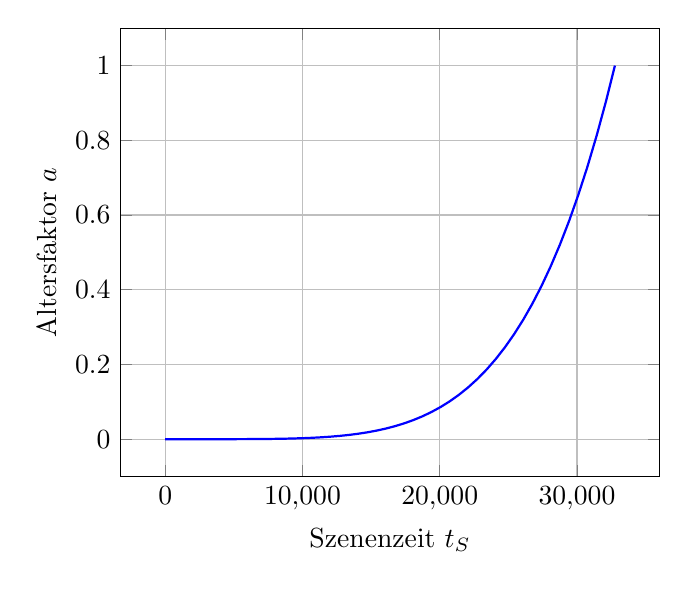
\begin{tikzpicture}
        \begin{axis}[
                ymin = -0.1,
                ymax=1.1,
                domain = 0:32768,
                samples=50,
                xlabel={Szenenzeit $t_S$},
                ylabel={Altersfaktor $a$},
                scaled x ticks = false,
                grid=both,
            ]
            \addplot[thick,blue]{(x/32768)*(x/32768)*(x/32768)*(x/32768)*(x/32768)};
        \end{axis}
    \end{tikzpicture}
    \captionof{figure}{Abhängigkeit des Altersfaktors $a$ von der Szenenzeit $t_S$ für die Datengenerierung.}
    \label{fig:age}
\end{center}

Die Verwendung der Parameter ist je nach Objekt unterschiedlich; während sie in Hauptobjekten häufig eingesetzt werden, nutzen Nebenobjekte diese eher selten. Dies liegt im Zusammenhang mit der Häufigkeit ihres Vorkommens in den Daten.


% -----------------------------------------------
\subsubsection{Hauptobjekte}
\label{sec:impl:daten:blender:hauptobjekte}

Als \textit{Hauptobjekte} werden diejenigen Objekte in der Szene beschrieben, die zentral für die Datenerstellung sind. Namentlich sind dies die Dartscheibe, die Dartpfeile und die Kamera.

\paragraph{Dartscheibe}
\label{sec:impl:daten:blender:hauptobjekte:dartscheibe}

Die Dartscheibe ist das komplexeste Objekt der Szene, da ihr Erscheinungsbild als zentrales Element der Bilder ausschlaggebend für die Komplexität und Variabilität der Daten ist. Aus diesem Grund ist sie mit einer Vielzahl an Parametern und Eigenschaften versehen. Sie ist gemäß der Richtlinien \quotes{Playing and Tournament Rules} der \ac{WDF} \cite{wdf-rules} erstellt. Dieses Regelwerk legt die Dimensionen und Abstände der Felder sowie etwaige Toleranzen fest. Auf dieses Regelwerk wurde sich in dieser Thesis bei der Arbeit mit Dartscheiben orientiert, Abweichungen durch esoterische Maße und Erscheinungsbilder von Dartscheiben, die nicht durch dieses Regelwerk gestützt sind, wurden für diese Arbeit nicht in Betracht gezogen. Die Parametrisierung der Scheibe ist in zwei Bereiche einzuteilen: Geometrie und Textur.

Die Geometrie der Dartscheibe ist durch die Regeln der \ac{WDF} zu großen Teilen vorgegeben. Um Alter und Abnutzung der Dartscheibe zu simulieren, wird der Deformationsgrad der Spinne\footnote{Als Spinne werden die Abgrenzungen zwischen den Feldern bezeichnet.} moduliert. Dazu wird der Parameter $t_S$ als Seed für eine 2D-Verschiebung der Mesh-Vertices anhand einer zusammenhängenden Noise-Textur verwendet und diese wird mit dem Parameter $a$ in ihrer Stärke moduliert. Dadurch weisen Dartscheiben mit einem hohen Altersfaktor $a$ eine größere Deformierung der Spinne auf während Dartscheiben mit einem geringen Wert von $a$ geringe bis keine Deformierung aufweisen. Ebenfalls von dem Altersfaktor beeinflusst wird die Art der Spinne: Während Spinnen neuer Dartscheiben aus dünnen Drähten bestehen, ist der Durchmesser dieser bei alten Dartscheiben größer und die Wahrscheinlichkeit, dass die Spinne mit weiteren Drähten zur Befestigung der Spinne auf der Scheibe versehen ist, steigt.

Der Großteil der variablen Parameter der Dartscheibe liegt jedoch nicht in der Geometrie, sondern in dem Material der Dartscheibe. Anhand unterschiedlicher Zufallsverteilungen, gestützt durch $t_S$ als Seed, werden die Farben der Felder, Abnutzung der Scheibe und Anzahl der Einstichlöcher im Sisal bestimmt.
Um realistische Materialien zu simulieren, werden unterschiedliche Imperfektionen in das Material eingearbeitet. Diese lassen sich in zwei Kategorien einteilen: Reine Farbänderungen und Farbänderungen, die eine Änderung der Normalen mit sich ziehen.

Zu der ersten Kategorie der Imperfektionen zählen kleine Haare und Staubpartikel, die sich auf der Dartscheibe ablagern. Diese sorgen für feine Verfärbungen und unterschiedliche Lichtbrechungen. Dazu kommen Spuren von Abnutzung, die je nach Alter unterschiedlich stark ausgeprägt sind. Diese Abnutzungen sind in Form von Kratzern und Abrissstellen zu erkennen.
Die zweite Kategorie der Imperfektionen sind Risse und Einstichstellen im Sisal. Durch seine Beschaffenheit reißt Sisal mit der Zeit, diese Risse werden sowohl durch Farbänderung als auch durch Einkerbungen in den Feldern simuliert. Weiterhin werden Einstichlöcher von Dartpfeilen simuliert und farblich hervorgehoben. Diese Faktoren sind ebenfalls abhängig vom Alter der Dartscheibe unterschiedlich stark ausgeprägt.

Mit zunehmendem Altersfaktor $a$ nimmt weiterhin die Farbsättigung der schwarzen und weißen Felder zu, wohingegen rote und grüne Felder an Sättigung verlieren und dunkler werden. Diese Anpassung der Feldfarben simuliert das Altern des Sisals der Dartscheiben, basiert auf Beobachtungen neuer und alter Dartscheiben. Darüber hinaus weisen alte Dartscheiben häufiger abgenutzte Zahlenringe auf, die sich durch Rost und Verfärbungen auszeichnen.

Alle diese Variabilitäten in den Dartscheiben sorgen für unterschiedliche Beschaffenheiten von Dartscheiben, die zufällig anhand eines Seeds generiert werden. Beispiele für simulierte Dartscheiben sind in \autoref{img:dartscheiben} gegeben. In der Abbildung sind drei Dartscheiben mit unterschiedlichen Altersfaktoren $a$ gegeben: \autoref{img:dartscheibe_neu} als neue Dartscheibe mit $a=0$, \autoref{img:dartscheibe_mittel} als Dartscheibe mit mittlerem Alter $a\approx0.5$ und \autoref{img:dartscheibe_alt} mit $a=1$.

\begin{figure}
    \centering
    \begin{subfigure}{0.3\textwidth}
        \centering
        \includegraphics[width=\textwidth]{imgs/dartscheibe_a=0.png}
        \caption{$a=0$}
        \label{img:dartscheibe_neu}
    \end{subfigure}
    \hfill
    \begin{subfigure}{0.3\textwidth}
        \centering
        \includegraphics[width=\textwidth]{imgs/dartscheibe_a=0.5.png}
        \caption{$a\approx0.5$}
        \label{img:dartscheibe_mittel}
    \end{subfigure}
    \hfill
    \begin{subfigure}{0.3\textwidth}
        \centering
        \includegraphics[width=\textwidth]{imgs/dartscheibe_a=1.png}
        \caption{$a=1.0$}
        \label{img:dartscheibe_alt}
    \end{subfigure}
    \caption{Dartscheiben mit unterschiedlichen Altersfaktoren.}
    \label{img:dartscheiben}
\end{figure}

\paragraph{Dartpfeile}
\label{sec:impl:daten:blender:hauptobjekte:dartpfeile}

Neben der Dartscheibe sind die Dartpfeile weitere Hauptobjekte. Im Gegensatz zur Dartscheibe ist ihre Geometrie weniger stark durch das Regelwerk der \ac{WDF} vorgegeben, sodass eine größere Variabilität geschaffen werden kann. Dartpfeile setzen sich aus \textit{Tip}, \textit{Barrel}, \textit{Shaft} und \textit{Flight} zusammen; für jedes dieser Teile existiert eine Gruppe an Objekten, die zufällig miteinander kombiniert und teilweise zufällig texturiert werden. Die unterschiedlichen Objekte der jeweiligen Klassen sind in \autoref{img:dartpfeil_teile} dargestellt. Diese Einzelteile sind inspiriert durch reale Dartpfeile. Bei dem Zusammensetzen werden Tip, Barrel und Shaft zufällig gestaucht oder gestreckt, um weitere Variabilität in die Dartpfeile zu integrieren. Für die Farben der Flights wird eine Basistextur zufällig gesampled. Zur Erstellung dieser Basistextur wurde die Bilderstellungs-KI von DeepAI genutzt \cite{deepai-image}. Darüber hinaus ist den Flights ein Altersfaktor zugewiesen, der den Grad der Verformung bestimmt. Je älter ein Pfeil ist, desto stärker kann er deformiert sein. In \autoref{img:dart_examples} sind einige Beispiele verschiedener Dartpfeile dargestellt. Zu erkennen ist in diesen die zufällige Wahl der Bestandteile und die Variation der Materialien.

\begin{figure}
    \centering
    \includegraphics[width=\textwidth]{imgs/darts.png}
    \caption{Bestandteile der Dartpfeile (von links nach rechts): Tips, Barrels, Shafts und Flights.}
    \label{img:dartpfeil_teile}
\end{figure}

\begin{figure}
    \centering
    \includegraphics[width=0.7\textwidth]{imgs/darts_examples.png}
    \caption{Darts Examples}
    \label{img:dart_examples}
\end{figure}

\paragraph{Kamera und Komposition}
\label{sec:impl:daten:blender:hauptobjekte:kamera}

Ein weiterer wichtiger Bestandteil der Szene sind die Kamera und die Komposition. Das Zusammenspiel dieser Bereiche ist daran ausgerichtet, Bilder zu rendern, die in ihrem Aussehen an Aufnahmen von Mobiltelefonen angelehnt sind. Dabei werden Blurring, Bloom, Lens Distortion und Film Grain simuliert, um Ungenauigkeiten von Handyaufnahmen zu simulieren. Die jeweiligen Ausprägungen dieser Nachverarbeitungsschritte wurden durch Analyse eigener Aufnahmen unterschiedlicher Kameramodelle eingestellt. Der Fokuspunkt der Kamera ist auf ein Objekt gelegt, das zufällig im Bereich um die Dartscheibe platziert wird. Weitere interne und externe Kameraparameter wie Bewegungsunschärfe, Auflösung oder Brennweite werden bei der Erstellung durch Skripte gesetzt, die in \autoref{sec:impl:daten:python} erläutert werden.

% -----------------------------------------------
\subsubsection{Nebenobjekte}
\label{sec:impl:daten:blender:nebenobjekte}

Neben den Hauptobjekten, die in nahezu allen Bildern zu sehen sind, existieren in der Szene weitere Objekte die zufällig erscheinen können.

\paragraph{Beleuchtung}
\label{sec:impl:daten:blender:nebenobjekte:licht}

Es werden unterschiedliche Arten der Beleuchtung eingesetzt. Dazu zählen Environment-Texturen, der Kamerablitz, ein Spotlight, Deckenlampen und ein LED-Ringlicht um die Dartscheibe herum. Die Environment-Texturen stammen von der Webseite PolyHaven und werden zufällig gewählt und in ihrer Stärke moduliert \cite{polyhaven}. Der Kamerablitz ist als helles Punktlicht modelliert, das wenige Zentimeter von der Kamera entfernt liegt. Dadurch ist eine realistische Ausleuchtung der Szene mit scharfem Schattenwurf in direkter Nähe der Objekte möglich. Weiterhin für scharfe Schatten sorgt ein Spotlight, das sich über der Kamera befindet und auf die Dartscheibe gerichtet ist. Diese Art der Beleuchtung wird im Strongbow's in Kiel verwendet, wo unter anderem Daten für diese Arbeit aufgenommen wurden. Deckenlampen wurden durch warme Leuchtstoffröhren in vergitterten Boxen modelliert, die in zwei Reihen entlang der Decke aufgereiht sind. Die Art der Beleuchtungen und ihre Ausprägungen werden nicht in der Szene festgelegt, sondern durch externe Skripte zur Erstellung der Daten.

\paragraph{Dartschrank und LED-Ring}
\label{sec:impl:daten:blender:nebenobjekte:cabinet}

Um die Dartscheibe herum können ein Dartschrank oder ein LED-Ring eingeblendet werden. Der LED-Ring besteht aus einem Zylinderförmigen Korpus, an dessen Vorderkante auf die Dartscheibe gerichtete LED-Lichter angebracht sind. Dieses Art des Ringlichts ist geläufig bei der Verwendung von Dartscheiben; die Farbe der LEDs werden, ebenso wie die Farbe des Rings, zufällig gewählt. Der Dartschrank ist mit einer Holztextur versehen, deren Sättigung und Helligkeit ebenfalls zufällig gewählt wird, und die Türen werden in einem zufälligen Winkel geöffnet.

Beide Objekte können nicht gemeinsam auftreten, da sie im selben Raum auftreten und ein gemeinsames Einblenden zu Überschneidungen der Objekte führen würde. Folglich ist entweder eines dieser Objekte oder keines vorhanden.

% ------------------------------------------------------------------------
\subsection{Python-Skript zur Randomisierung von Parametern}
\label{sec:impl:daten:python}

Das Rendern der Szene geschieht nicht aus Blender heraus, sondern wird durch die Python-Bibliothek \textit{bpy} gesteuert. Durch diese Bibliothek ist es möglich, die Szene deskriptiv und ohne GUI zu manipulieren und zu steuern. Das Setzen von Parametern und das gezielte Anordnen der Objekte in der Szene wird auf diese Weise erzielt.

\paragraph{1. Generelles Setup}
\label{sec:impl:daten:python:setup}

Der erste Schritt zur Erstellung einer Szene für das Rendern eines Samples ist die Randomisierung des globalen Szenenparameters $t_S$. Dieser wird von den Objekten als Seed zur Erstellung von Zufallswerten und als Altersfaktor genutzt. Er wird uniform zwischen der minimalen und maximalen Szenenzeit gewählt.

\paragraph{2. Beleuchtung und Umgebungsobjekte}
\label{sec:impl:daten:python:licht}

Die Beleuchtung der Szene ist ein mehrschrittiger Prozess, in dem eine Abstimmung der unterschiedlichen Beleuchtungsmöglichkeiten geschaffen wird, um eine realistische Verwendung von Lichtquellen zu erzielen. Der erste Schritt der Beleuchtung ist die Wahl der Umgebungsbeleuchtung durch die Environment-Textur. Diese wird zufällig aus einem Pool von >200 HDRIs und einer Intensität $I_{HDRI} \in [0, 1]$ gewählt. Zudem wird sie zufällig um die Z-Achse rotiert, um die Anzahl der Dopplungen gleicher Hintergründe weiter zu minimieren. Die Intensität $I_{HDRI}$ bestimmt die Wahrscheinlichkeit der Aktivierung von Kamerablitz, Spotlight und Deckenbeleuchtung. Je dunkler die Umgebung, desto wahrscheinlicher ist die Existenz weiterer Beleuchtungen.
Weiterhin wird mit einer Wahrscheinlichkeit von $5\%$ der Dartschrank eingeblendet und mit einer Wahrscheinlichkeit von $15\%$ das Ringlicht. Diese Fälle schließen sich gegenseitig aus, sodass lediglich eines von beiden Objekten existieren kann.
Sind weder Kamerablitz, Spotlight oder der LED-Ring aktiviert, ist die Deckenbeleuchtung gesichert als Rückfall-Lichtquelle aktiviert, um nicht beleuchtete Szenen auszuschließen.

\paragraph{3. Text}
\label{sec:impl:daten:python:text}

Um den Rand der Dartscheibe befinden sich zwei Textobjekte, \textit{top} und \textit{bottom}. diese Objekte befinden sich auf gegenüberliegenden Seiten und sind jeweils um 180° voneinander entfernt. Die Schriftart der Texte stammt aus einem Pool von 16 Schriftarten. Diese wird zufällig ausgewählt. Die angezeigten Texte stammen aus einer Liste von 130 Texten für \textit{top} und 139 Texten für \textit{bottom}, die zufällig miteinander kombiniert und um die Dartscheibe rotiert werden.

\paragraph{4. Dartpfeile}
\label{sec:impl:daten:python:pfeile}

Die Anordnung der Dartpfeile auf der Dartscheibe ist ein mehrschrittiger Prozess. In erster Instanz wird je Pfeil entschieden, ob dieser existiert oder nicht. Die Wahrscheinlichkeit der Existenz beläuft sich auf 70\%. Wird ein Pfeil angezeigt, wird er anhand einer typischen Darts-Heatmap auf der Dartscheibe positioniert. Diese Heatmap, visualisiert in \autoref{img:heatmap}, ist orientiert an einer Auswertung von Darts 1 \cite{heatmap} und spiegelt ein typisches Trefferbild wider. Die Platzierung der Dartpfeile wird nach Festlegung einer Position derart korrigiert, dass sie weder mit der Spinne noch mit anderen Dartpfeilen kollidieren. Sobald die Position final festgelegt ist, werden die Pfeile zufällig nach dem Vorbild realer Muster rotiert. Anhand der Platzierungen auf der Dartscheibe wird die Punktzahl des Wurfs bestimmt.

\begin{figure}
    \centering
    \includegraphics[width=0.8\textwidth]{imgs/heatmap.png}
    \caption{Darts-Heatmap für das Generieren von Daten. Bereiche mit durchschnittlicher Trefferwahrscheinlichkeit sind in gelb und grün markiert während in blau unwahrscheinliche Trefferbereiche und in rot wahrscheinliche Bereiche dargestellt sind.}
    \label{img:heatmap}
\end{figure}

\paragraph{5. Kamera}
\label{sec:impl:daten:python:kamera}

Zur Einstellung einiger Kameraparameter existieren Objekte in der Szene, durch die bestimmte Randbedingungen festgelegt werden. Zum einen existiert ein Objekt, das den Bereich festlegt, in dem die Kamera platziert wird. Der Kamerabereich ist parametrisiert durch:
\begin{itemize}
    \item Abstand zur Dartscheibe $d \in [60, 150]\text{cm}$
    \item Höhe $h \in [160, 220]\text{cm}$
    \item seitliche Distanz zur Dartscheibe $|d_{x\_max}| < 60\text{cm}$
    \item maximaler seitlicher Winkel $|\phi_z| < 120\degree$
    \item maximaler vertikaler Winkel $|\phi_x| < 60\degree$
\end{itemize}

Diese Distanzen und Winkel beziehen sich auf die Mitte der Dartscheibe, die sich nach dem Regelwerk der \ac{WDF} in einer Höhe von 207cm befindet. Eine Darstellung des Bereichs der Kameraplatzierung ist mit \autoref{img:camera_space} gegeben.

\begin{figure}
    \centering
    \includegraphics[width=0.8\textwidth]{imgs/camera_space.png}
    \caption{Visualisierung des Bereichs, in dem die Kamera platziert werden kann.}
    \label{img:camera_space}
\end{figure}

Nachdem die Kamera zufällig in dem vorgegebenen Bereich Platziert ist, wird sie auf die Dartscheibe gerichtet und ihr Fokuspunkt wird zufällig auf der Dartscheibe positioniert mit einer normalverteilten Verschiebung von der Dartscheibe entfernt. Darüber hinaus existiert eine Wahrscheinlichkeit von $10\%$, dass die Kamera mit Bewegungsunschärfe versehen wird.

Sobald alle externen Kameraparameter gesetzt sind, werden die internen Kameraparameter gewählt. Die Brennweite wird anhängig von dem Abstand der Kamera zur Dartscheibe zwischen 18 und 60mm gesetzt und die Öffnung der Linse wird ebenfalls in Abhängigkeit der Distanz zur Dartscheibe auf einen Wert zwischen 1.8 und 5 gesetzt, wodurch der F-Stop der Kamera bestimmt wird. Das Bildformat der Kamera wird zufällig aus einer Liste gängiger Bildformate von Mobiltelefonen gesetzt. 70\% aller Bilder werden im Hochformat, 30\% aller Bilder im Querformat aufgenommen und die Auflösung der Bilder wird zufällig zwischen 1000 und 4000px entlang der längeren Seite gesetzt. Die Belichtung der Kamera wird in einem Wertebereich zwischen 0.2 und 1.0 gesetzt. Diese spezifischen Bereiche der Kameraparameter wurden durch Metadatenanalyse eigener Aufnahmen und subjektive Bewertung von gerenderten Bildern festgelegt.


\paragraph{6. Rendering}
\label{sec:impl:daten:python:render}

Durch die Verwendung der Bibliothek \textit{bpy} ist über das Setzen unterschiedlicher Parameter hinaus auch das Rendern von Bildern möglich, ohne die Notwendigkeit einer graphischen Benutzeroberfläche. Dadurch ist es möglich, automatisiert Daten zu erstellen. Neben dem Rendern der Dartscheibe werden weitere Masken von Objekten gerendert. Diese dienen der Identifizierung unterschiedlicher Objekte im Post-Processing.

Als binäre Masken zur Identifizierung und Lokalisierung unterschiedlicher Objekte in dem Bild werden die Dartpfeile, die Frontseite der Dartscheibe, Orientierungspunkte zur Entzerrung der Dartscheibe und die Einstichpunkte der Dartpfeile exportiert. Diese Masken ermöglichen die Bestimmung relevanter Informationen in den gerenderten Bildern.

% ------------------------------------------------------------------------
\subsection{Post-Processing der Daten}
\label{sec:impl:daten:postprocess}

Nach dem Rendern des Bildes und der Masken geschehen weitere Schritte des Post-Processings. Aus der Maske der Orientierungspunkte wird eine Homographie zur Entzerrung der Dartscheibe abgeleitet, durch die die Dartscheibe normalisiert wird. Dieses normalisierte Bild der Dartscheibe ist der Input für das später trainierte Neuronale Netz zur Lokalisierung der Dartpfeile. Die Maske der Dartpfeil-Einstichstellen wird genutzt, um die Positionen der Pfeilspitzen zu lokalisieren. Dies erfolgt sowohl auf dem gerenderten Bild als auch auf dem entzerrten Bild, indem die Entzerrungstransformation auf die Maske angewandt wird. Darüber hinaus werden weitere Informationen zur Geometrie der Dartscheibe und Überschneidungen und Verdeckungen der Dartpfeile errechnet und gespeichert. Diese sind für die Evaluierung des Systems relevant.

% -------------------------------------------------------------------------------------------------
% DARTSCHEIBE

\section{Dartscheiben-Alignment}
\label{sec:impl:cv}

- Paper: CNN für Orientierungspunkte + Dartpfeile
- Problem: Wenig Orientierungspunkte -> Verdeckung = unbrauchbar
- Lösungsvorschlag laut Paper: Mehr Orientierungspunkte fitten
- Lösungsvorschlag laut Justin: Computer Vision
- Dartscheiben sehr markantes Aussehen -> gut für CV
- Nicht alle Probleme müssen mit KI gelöst werden; Blackbox, deren Grenzen nicht klar definierbar sind
- Umsetzung komplexer als antizipiert, aber robuste Lösung gefunden

\subsection{Vorverarbeitung}
Bild laden + skalieren

\subsection{Kantenerkennung}
Kanten erkennen + Skeletonization

\subsection{Linienerkennung}
HoughLines

\subsection{Mittelpunkt-Extraktion}
Linien binnen + Überlagern + Mittelpunkt extrahieren

\subsection{Linienfilterung}
Linien nach Distanz zu Mittelpunkt filtern

\subsection{Feldlinien-Berechnung}
Linien finden + Linien an Punkten ausrichten

\subsection{Mittelpunkt-Verfeinerung}
Neue Linien -> besserer Mittelpunkt

\subsection{Feldlinien-Winkelentzerrung}
Bekannte Winkel -> Ausrichten (viel Mathe)

\subsection{Orientierungspunkte identifizieren}
Logpolar + Corner Detection + Surroundings + SSIM

\subsection{Einordnen der Orientierungspunkte}
Distanzen etc.

\subsection{Homographiefindung durch Orientierungspunkte}
OpenCV, aber mit eigenem RANSAC-Ansatz

\subsection{Undistortion + Alignment}
Originalbild mit Matrizen entzerren + Croppen

% -------------------------------------------------------------------------------------------------
% DARTPFEILE

\section{Dartpfeil-Erkennung}
\label{sec:impl:ki}

TODO

Vortrainiertes CNN-Backbone
Erkennung der Dartpfeil-Spitzen
Klassifizierung der Dartpfeile in Felder?
